% Chart B: Unfreeze-N sweep — illustrates the val/Kaggle inversion.
% Source: src_experiments/014_unfreeze_sweep/summary.md and chart_data.js UNFREEZE_SWEEP.
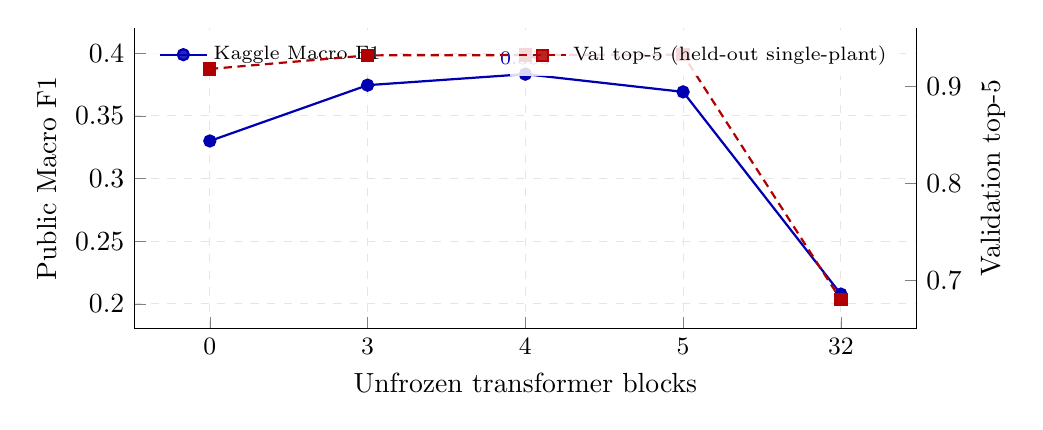
\begin{tikzpicture}
  \begin{axis}[
      width=0.95\linewidth, height=5.4cm,
      xlabel={Unfrozen transformer blocks},
      ylabel={Public Macro F1},
      ymin=0.18, ymax=0.42,
      ytick={0.20,0.25,0.30,0.35,0.40},
      symbolic x coords={0, 3, 4, 5, 32},
      xtick=data,
      xticklabel style={font=\small},
      ylabel near ticks,
      axis y line*=left,
      axis x line*=bottom,
      grid=major, grid style={dashed,gray!20},
      enlarge x limits=0.12,
      every axis plot/.append style={thick},
      legend style={at={(0.02,0.98)}, anchor=north west,
                    font=\scriptsize, draw=none, fill=white, fill opacity=0.85,
                    text opacity=1},
    ]
    \addplot+[mark=*, color=blue!70!black, mark options={fill=blue!70!black}]
      coordinates {(0,0.33000) (3,0.37455) (4,0.38333) (5,0.36919) (32,0.20777)};
    \addlegendentry{Kaggle Macro F1}
    \node[anchor=south, font=\scriptsize, color=blue!70!black]
      at (axis cs:4,0.38333) {0.383};
  \end{axis}
  \begin{axis}[
      width=0.95\linewidth, height=5.4cm,
      ymin=0.65, ymax=0.96,
      ytick={0.70,0.80,0.90},
      ylabel={Validation top-5},
      symbolic x coords={0, 3, 4, 5, 32},
      xtick=\empty,
      axis y line*=right,
      axis x line=none,
      ylabel near ticks,
      enlarge x limits=0.12,
      every axis plot/.append style={thick, densely dashed},
      legend style={at={(0.98,0.98)}, anchor=north east,
                    font=\scriptsize, draw=none, fill=white, fill opacity=0.85,
                    text opacity=1},
    ]
    \addplot+[mark=square*, color=red!70!black, mark options={fill=red!70!black, solid}]
      coordinates {(0,0.9180) (3,0.9320) (4,0.9323) (5,0.9327) (32,0.6800)};
    \addlegendentry{Val top-5 (held-out single-plant)}
  \end{axis}
\end{tikzpicture}
